\section{相关技术与理论基础}

\subsection{医学图像语义分割基础}

图像分割任务可以分为两个不同的任务类别:语义分割任务和实例分割任务\cite{azad2024}。语义分割是像素级图像分割,图像中的每个像素点都有一个对应的类别,语义分割任务则需要尽量正确预测每个像素点的类别。实例分割在语义分割任务的基础上,需要将同类别的像素分类为不同的对象实例,即同类不同例,如图~\ref{fig:seg}所示。基于医学图像的语义分割任务则是指利用计算机视觉技术去分析和处理2D或3D医学图像,达到将人体器官、软组织和病灶体进行分割、提取,三维重构和展示的目的\cite{liu2021}。

\begin{figure}[htbp]
    \centering
    \subfloat[原图]
    {
        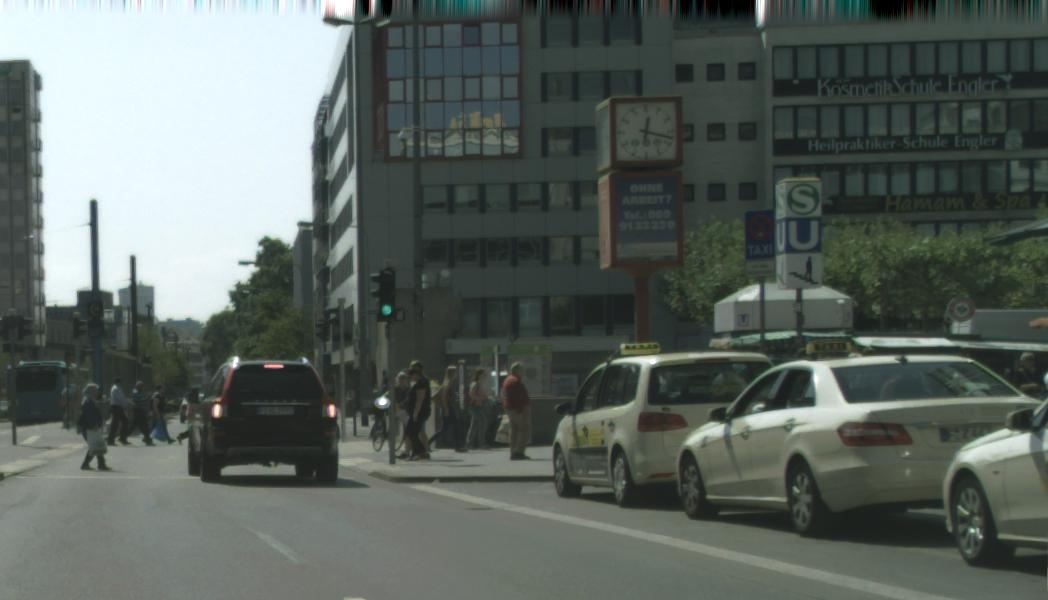
\includegraphics[width=0.3\textwidth]{fig/img_seg.jpg}
    }
    \subfloat[语义分割图]
    {
        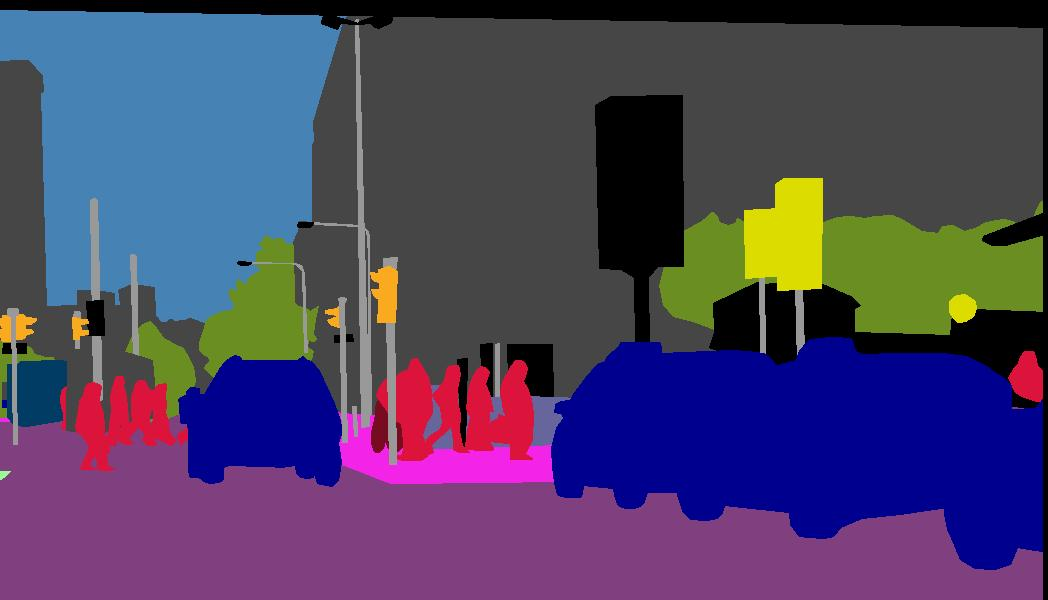
\includegraphics[width=0.3\textwidth]{fig/semantic_seg.jpg}
    }
    \subfloat[实例分割图]
    {
        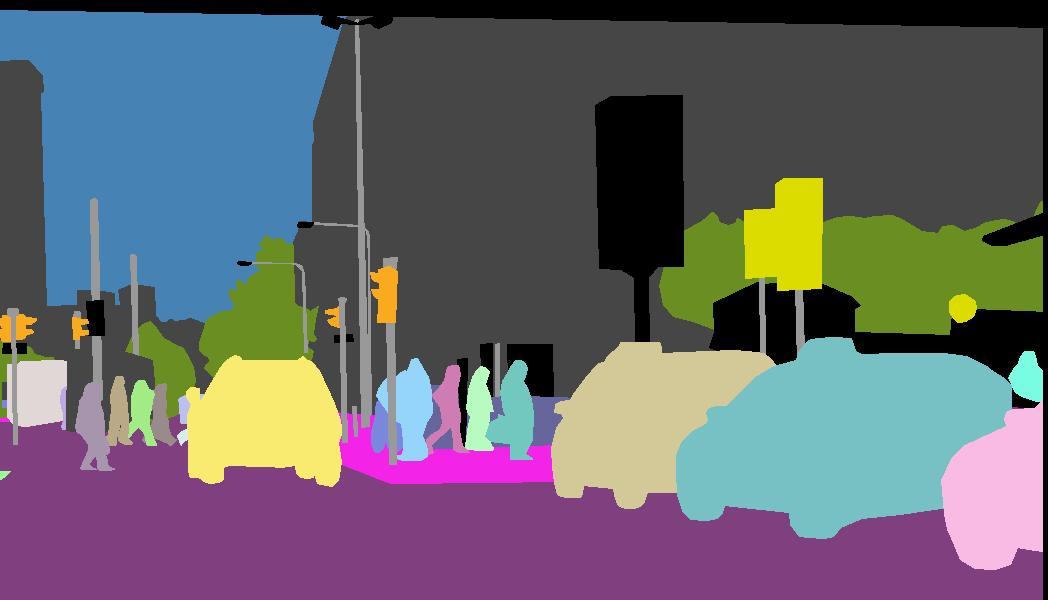
\includegraphics[width=0.3\textwidth]{fig/instance_seg.jpg}
    }
    \caption{语义分割与实例分割对比示意图\cite{kirillov2019}}
    \label{fig:seg}
\end{figure}

\subsubsection{医学图像特点}

% 考虑是否引用第一章某处内容
医学图像作为临床诊断与治疗决策的重要依据,具备区别于自然图像的一系列独特特点:

\begin{enumerate}
    \item 多模态性: 
    多模态性是医学图像最本质的特征之一,不同成像技术基于各自的物理机制产生图像,导致图像在分辨率、对比度、噪声特性等方面具有显著差异。例如,CT图像通过X射线衰减反映组织的密度信息,表现为良好的骨骼成像与高密度区域识别能力;MRI通过核磁共振原理获取图像,具有出色的软组织对比度,常用于脑部、脊髓及肿瘤成像。
    
    \item 高噪声和低对比度:
    相较于多数自然图像的高清晰度和高对比度,高噪声与低对比度问题在医学图像中普遍存在。受限于成像设备、器官运动等因素,医学图像常伴有伪影与模糊,如MRI中常见的运动伪影与磁敏感伪影、CT中的金属伪影。低对比度则体现在图像的病灶区域与周围正常组织在灰度分布上高度重叠,如肝脏与肿瘤组织;也常出现多个器官重叠或粘连的情况,如腹部CT图像中的脾脏与左肾的接触区域、脑白质与灰质区域。
    
    \item 解剖结构的拓扑复杂:
    自然图像的物体通常具有清晰空间分层(如“前景-背景”),而在医学图像中器官和组织常呈现多层嵌套(如肠管缠绕、血管穿透脏器)和动态形变(如呼吸导致的肺位移)。同时,自然物体的形状相对稳定,而人体解剖结构会因为个体差异、病理状态产生巨大形态变异,例如前列腺癌患者的腺体体积可膨胀至正常值的3倍。
    
    \item 数据获取和标注困难:
    医学图像的数据获取和标注远高于自然图像。成像成本高、病人隐私问题、罕见病例少等等因素导致医学图像的数据量通常只有数百数千张,甚至更少。同时高质量的可用于图像分割的医学图像需要具有多年经验的临床专家进行逐像素级精细勾画,且不同医生间的标注标准与经验存在差异,导致“标注者间差异”现象普遍存在。

\end{enumerate}

% 附图:自然图像+高噪声医学图像+复杂拓扑结构医学图像

上诉特点使得医学图像相较于自然图像有更高的复杂性,对其的自动分割任务不仅要求模型具备强大的特征表达与结构建模能力,还需应对多种极具挑战性的实际问题。

\subsubsection{医学图像语义分割挑战}

在数据具有多模态性和获取标注困难的情况下,跨模态泛化能力成为了衡量模型在医学图像语义分割性能的关键评估指标,一个鲁棒的能够适用于医学图像语义分割任务的模型应当能够在这种模态一致性不足和低数据量的情况下维持良好稳定的性能。而低对比度和解剖结构复杂的特点,对模型提出了更强的捕捉高分辨率细节并维持边缘清晰度的能力要求,许多早期病灶(如肺部结节、肝癌早期病变)和器官(如视网膜微血管)在图像中的所占面积比例极小,容易在下采样的过程中被忽略和抹除,模型需要能够在这种情况下对小目标进行精细分割。

除了受医学图像固有的复杂性影响,高实时性也是医学图像语义分割模型应当具备的能力,同时也是决定模型能否落地应用的重要门槛。在术中导航、放疗定位、超声实时识别等高时效性场景中,模型不仅要保证分割准确,还需在极短时间内完成推理,这同时也对模型的计算复杂度与硬件适配能力提出了极高的要求。

综上,面向于医学图像的语义分割算法和模型不仅有高分割精度和跨模态泛化的能力要求,还需要面对高实时性等的性能挑战。这种挑战也促使了大量的研究者进入医学图像语义分割领域进行探索,提出了诸多有效的分割算法和创新的网络结构与优化策略,这些工作将在下文中进行全面的介绍。

\subsection{传统分割方法概述}

% 结合医学图像中的应用阐述适用性和局限性,同时:删减内容!删减内容!

在相当长的一段时间内,基于边界或区域的传统分割技术作为医学图像分析的基础,提供了一系列复杂性和适用性有所不同的方法。基于区域的分割方法依赖图像的空间特征,例如灰度和纹理。基于边界的分割方法则主要使用梯度信息来确定目标的边界。包括阈值分割、边缘检测、区域生长及聚类分割等在内的传统分割方法在很多场合下已被证明有效\cite{xu2024},但在跨模态、跨患者场景中传统方法存在较大的局限性(详见第一章1.1节)。接下来的内容将对阈值分割、边缘检测和聚类分割这三种最具代表性且广泛应用的传统分割方法进行概述总结。

\subsubsection{阈值分割}

阈值分割是图像分割中最基础、最广泛使用的技术之一,其核心思想是通过设定一个或多个灰度阈值,将图像像素进行二分类(如前景和背景):

\begin{equation}
B(x, y)=\left\{\begin{array}{ll}1, & \text { if } I(x, y) \geq T \\ 0, & \text { if } I(x, y)<T\end{array}\right.
\end{equation}

其中,$I(x, y)$表示图像在坐标$(x, y)$处的像素值,$B(x, y)$表示二元图像在坐标$(x, y)$处的像素值,$T$则是阈值。在图像处理中,阈值分割方法又可以细分为两大类:全局阈值法和局部阈值法。

全局阈值法假设整幅图像的背景与前景有明显的灰度差异,因此通过应用一个统一的阈值$T$来对图像进行分割。比较著名的全局阈值算法包括:Otsu法、迭代法和最小误差法。Otsu法通过最大化类间差异选取最优阈值;迭代法则初始估计一个阈值,然后迭代更新前景和背景的平均灰度值来计算新阈值直至收敛;最小误差法在基于图像前景和背景的像素灰度值呈正态分布的假设前提下,通过计算各分割区域的概率密度函数得到总分类误差并使误差最小化确定阈值。全局阈值法在图像灰度分布较均匀、对比度明显时表现良好,且计算成本低易于实现和集成到实时系统。但是,该方法在光照不均或对比度不明显的情况下分割效果差,同时也不适用于复杂背景或多目标图像分割。

相对于全局阈值法,局部阈值法假设图像具有不均匀的光照,因此针对每个像素的局部领域单独计算阈值$T$。较为常见的局部阈值算法包括:Niblack算法和Sauvola。Niblack通过计算每个像素上特定窗口内像素值的局部平均值和标准偏差,并利用平均值评估局部亮度、标准偏差衡量对比度和纹理来动态设定阈值:$ T=\mu+k \sigma $。Sauvola则在Niblack的基础上进行改进,将标准偏差的动态范围R引入阈值计算:$ T=\mu\left[1+k\left(\frac{\sigma}{R}-1\right)\right] $,从而更好地处理变化的背景和光照条件。局部处理使得局部阈值法能处理光照不均、阴影遮挡的情况,提高了图像细节的保留能力,使其能适用于安全监控、指纹识别等对细节要求较高的场景。但是同时,其计算复杂度也变得更高、运行时间较长,而且在噪声较大的区域容易误判。

\subsubsection{边缘检测}

% 记得插入参考文献

边缘是是指两个均匀区域之间的边界,表现为图像中像素强度的局部突变。而边缘检测的核心就在于识别定位图像中像素强度突变的位置。在基于边缘的分割方法中,首先检测图像中目标物体的轮廓以及物体与背景之间的边界,随后通过连接边缘形成物体边界以实现目标区域分割。

在基于边缘的图像分割技术中,整个过程通常按一系列明确的步骤展开。首先进行图像预处理,为后续分析奠定基础;随后执行边缘检测这一关键步骤,识别图像中的潜在边界;接着应用非极大值抑制技术对检测结果进行精细化处理,强化显著边缘的同时抑制微弱响应;然后通过阈值处理将梯度图二值化,实现边缘与非边缘的明确区分;之后是后处理阶段,通过填补间断或平滑不规则边缘进一步优化分割结果;最终依据上述步骤所得的边缘信息完成图像的区域分割。

图像边缘具有两个基本特性:方向与幅值。沿着边缘方向,像素值的变化往往较为平缓;而在垂直于边缘方向,像素值的变化则较为剧烈。基于这一特性,边缘检测常应用一阶和二阶微分算子来描述和检测图像中的边缘。

常见的一阶微分算子包括Roberts交叉算子、Prewitt算子、Sobel算子以及Canny边缘检测器,这些算子通过突出图像中像素强度的梯度变化来实现边缘检测。而二阶微分算子如Laplacian算子和高斯拉普拉斯算子同样被广泛采用。这些算子通过将特定模板与图像像素值矩阵进行卷积运算,精确计算各像素点的梯度变化或曲率,从而提取边缘特征。

如表~\ref{tab:edge_detectors}所示,不同的边缘检测算子具有各自的优势与局限性,适用于不同的应用场景。例如,Roberts交叉算子因其核尺寸小而具有计算简单、速度快的优势,特别适用于低噪声图像,但其对噪声敏感且在边缘定位精确方面表现仅达中等水平。

\renewcommand{\tabularxcolumn}[1]{m{#1}}
\newcolumntype{C}{>{\centering\arraybackslash}X}
\begin{table}[!htbp]
\centering
\caption{不同边缘检测算子的优缺点比较}
\label{tab:edge_detectors}
\begin{tabularx}{\textwidth}{@{}C C C@{}}
\toprule
\textbf{算子} & \textbf{优点} & \textbf{缺点} \\
\midrule
Roberts & 计算简单 & 对噪声敏感,边缘定位不准 \\
\addlinespace
Prewitt & 对边缘方向敏感 & 对噪声敏感,边缘较模糊 \\
\addlinespace
Sobel & 抑制噪声 & 边缘易过平滑\\
\addlinespace
Canny & 边缘检测精度高,抗噪性强 & 计算复杂,依赖参数调优\\
\addlinespace
Laplacian & 能定位边缘中心 & 抗噪性极差,无方向信息 \\
\addlinespace
高斯–拉普拉斯算子 & 抗噪性强且边缘定位准 & 计算量大,可能丢失细边缘 \\
\bottomrule
\end{tabularx}
\end{table}


Prewitt算子与Sobel算子均采用像素邻域差分法进行边缘检测。其中,Prewitt算子对边缘方向具有更高的敏感性,而Sobel算子则通过改进的噪声抑制能力获得更优性能,但代价是可能导致边缘轻微模糊。Canny算子作为多阶段边缘检测算法的典型代表,以高精度著称,不仅能有效抑制噪声干扰,还可实现边缘的准确定位,但其计算复杂度显著高于其他算子。

基于二阶导数的Laplacian算子对图像细节具有突出增强作用。尽管该算子易受噪声影响,但在细微特征增强方面表现卓越。高斯拉普拉斯算子通过高斯平滑预处理与Laplacian算子的协同作用,有效降低了噪声干扰,特别适用于噪声敏感环境下需要精确定位边缘的应用场景。

\subsubsection{聚类分割}

基于聚类的方法技术是图像分割的重要工具,通过将具有相似特征的像素划分至不同的簇中,从而实现有效分类。数据聚类的基本思想是通过预设的相似性或相异性度量,系统地将数据点划分为若干簇。在此过程中,每个簇被赋予一个标签,以确保同一簇内元素的相似性显著高于不同簇间元素的相似性。为系统地梳理聚类方法的理论框架,Fraley与Raftery提出了一个分类体系,将聚类技术划分为两大类:层次化聚类与划分式聚类。

在层次聚类方法中,簇的生成通常通过一种迭代式的模式划分过程实现,该过程可以采用自顶向下或自底向上的策略。这类算法通过构建一种二叉树状的数据结构——树状图来完成聚类任务。按照操作方式的不同,层次聚类可进一步分为两大类:凝聚型层次聚类与分裂型层次聚类。凝聚型层次聚类从最精细的层级开始,每个簇仅包含单一数据实体。该方法通过逐步合并相邻簇对,自底向上构建层次化结构。相反,分裂式层次聚类采用自上而下的策略,将包含所有实体的完整簇系统性地分解为更小的子簇,直至每个实体独立成簇或达到预定义终止准则。

尽管层次聚类方法具有良好的可解释性与层级结构建模能力,但其存在若干显著缺陷。首先,该类方法采用贪心策略,一旦某个样本被分配至某一簇,其归属将不会被重新评估,导致错误分类无法修正,鲁棒性较差,尤其在存在噪声或离群点的情形下更为明显。此外,层次聚类并不以优化某一全局目标函数为导向,在处理簇间重叠时表现不佳,降低了聚类的准确性。此外,层次聚类通常需要预先设定簇的数量或终止条件,这在实际应用中往往较难把握,影响聚类结构的自适应性。该方法也容易偏向形成球形簇结构,对于复杂空间分布的聚类任务可能导致结构失真。更重要的是,层次聚类的计算复杂度通常较高,随着样本规模增加,其在大规模数据场景下的可扩展性受到限制。

划分式聚类方法通过优化目标函数,将数据样本划分为若干个彼此独立的簇,从而增强簇内样本间的相似性,并尽可能降低簇间差异。该方法通过计算每个数据样本与不同簇之间的相似度,以最小化簇内相似性准则作为目标,评估聚类结果的有效性,从而寻求最具代表性的聚类配置。

与层次聚类类似,划分式聚类也通常要求预先指定簇的数量。该方法的一大特点在于:每个样本都被强制分配至某一特定簇中,即使某些样本距离所属簇中心较远,这在含有噪声或离群点的数据集中可能导致簇形严重失真,降低分割精度。根据分配方式可进一步分为硬聚类和软聚类两种。硬聚类,如最为经典的k-means算法,每个数据点仅归属于一个簇;而软聚类,如模糊c均值算法,允许每个数据点以不同隶属度隶属于多个簇。

与层次聚类不同,划分式聚类的主要优势在于其具备迭代优化能力,即通过多次更新簇中心与样本分配,不断提升聚类质量,从而更有效适应数据结构的变化。然而,这类方法也存在一系列局限性。首先,它们缺乏对簇结构的明确描述,严重依赖于事先设定的簇数,不具备自动确定最优聚类数目的能力;其次,对初始条件极为敏感,不同的初始簇中心选择可能导致截然不同的聚类结果。此外,在样本分布不均衡或非凸形状情况下,划分式聚类方法的表现明显下降,尤其容易受噪声与异常值的干扰。所以,尽管划分式聚类在优化性与计算效率上具备一定优势,但其在鲁棒性、自适应性与非理想分布处理能力方面存在不足,需结合实际任务特性合理选用。

\subsection{基于深度学习的语义分割技术}

深度学习作为机器学习与人工智能领域的重要研究方向,其核心在于通过深度神经网络模拟人脑学习机制,从海量数据(语音、文本、图像等)中以无监督方式自动提取特征表征。神经网络通过大量互连的神经元,从结构、实现机理和功能上模拟人脑神经网络,每个神经元可视为基础信息处理单元,通过层级化连接形成完整的网络架构\cite{qiu2020nndl}。该架构的出现使得端到端图像处理成为可能,当网络隐层扩展至多层结构时即形成深度学习范式。为解决深度网络训练难题,研究者提出逐层初始化与批量优化策略,推动深度学习成为当前智能化时代的核心技术并引发广泛研究热潮。在计算机视觉领域,深度学习已成功应用于数据降维、手写体识别、模式识别等方向,尤其在图像识别、图像修复、图像分割、目标追踪及场景解析等任务中展现出卓越性能。

\subsubsection{卷积神经网络}

卷积神经网络是深度学习与图像处理技术相结合的经典模型,作为深度学习技术领域最具代表性的神经网络之一,其在图像分析与处理领域取得了诸多突破性进展。在学术界广泛使用的标准图像标注集ImageNet上,基于卷积神经网络的特征提取与分类、模式识别等研究成果丰硕。

1962年Hubel等人\cite{hubel1962}通过生物学研究表明,大脑中视觉信息从视网膜传递是通过多级感受野激发完成的,并首次提出了感受野概念。基于感受野概念,1980年Fukushima\cite{fukushima1980}提出了神经认知机,被视为卷积神经网络的首次实现网络。与全连接层前馈网络不同的是,卷积神经网络通过交叉堆叠卷积层、池化层和全连接层形成前馈神经网络。大量的卷积层和池化层使得网络可以共享前层网络不同位置的特征映射权重,并利用空间相对关系来大大减少网络的参数量。同时,结构特性带来的一定程度上的平移、缩放和旋转不变性,使得卷积神经网络在图像和视频分析任务上具有远超其他神经网络模型的准确率\cite{qiu2020nndl}。

卷积神经网络通过卷积核(Convolution Kernel)对输入数据完成卷积操作,采用卷积代替全连接反馈网络的全连接,就构成了卷积神经网络的卷积层。在图像处理中最常见的卷积操作是二维卷积:

\begin{equation}
    \boldsymbol{O}=\boldsymbol{K} * \boldsymbol{I}
\end{equation}

其中$*$表示二维卷积运算,如图~\ref{fig:2dcnn}所示。$I$和$K$都是二维张量,$K$表示二维卷积核,$I$表示输入的二维图像数据。

\begin{figure}[htbp]
    \centering
    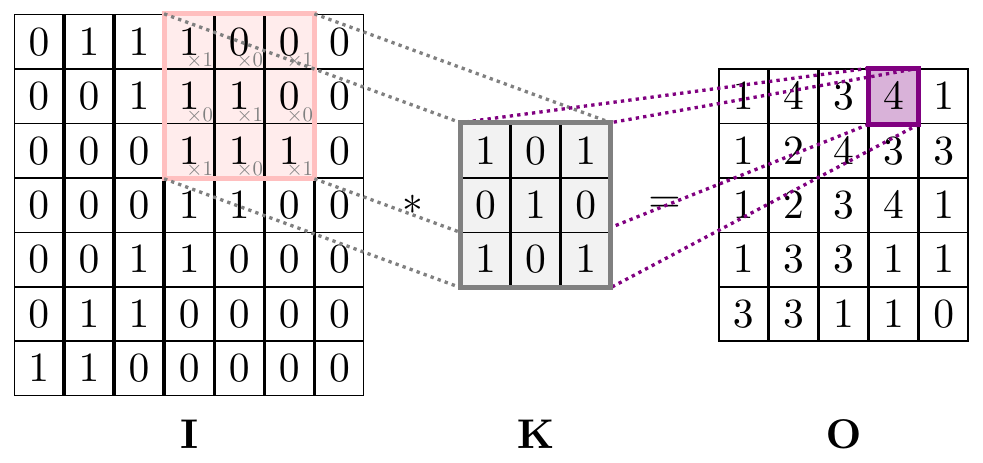
\includegraphics[width=\textwidth]{fig/2dcnn-1.png}
    \caption{二维卷积运算}
    \label{fig:2dcnn}
\end{figure}

对于一个有$l$层卷积层的卷积神经网络,第$l$层的输出$\boldsymbol{o}^{(l)}$为第$l-1$层的输出活性值$\boldsymbol{a^{(l-1)}}$和卷积核$\boldsymbol{w^{(l)}}$的卷积:

\begin{equation}
    \boldsymbol{o}^{(l)}=\boldsymbol{w}^{(l)} \otimes \boldsymbol{a}^{(l-1)}+b^{(l)}
\end{equation}

其中卷积核$ \boldsymbol{w}^{(l)} \in \mathbb{R}^{K} $为可学习的权重向量,$b^{(l)} \in \mathbb{R}$为可学习的偏置\cite{qiu2020nndl}。

\subsubsection{U-Net网络}


\subsection{模型评估指标}